\documentclass{article}
\usepackage{spconf,amsmath,epsfig}
\usepackage{graphicx}

\pagestyle{empty}
\begin{document}\sloppy

\title{
Selective Removal of Extraneous Photographs
}

\name{K. Armin Samii, Allison Carlisle, Uliana Popov, James Davis}
\address{[ksamii,acarlisl]@ucsc.edu,[uliana,davis]@soe.ucsc.edu}

\maketitle	
\begin{abstract}
In this paper, we propose a method for selecting the most representative high-quality images from a set of user photographs. To prevent redundancy arising from many similar images, we find all sets of near-duplicates. We then rank images based on three technical qualities: exposure, blur, and color harmony. Finally, we provide an ordering of the images which accounts for both quality and redundancy. Our goal is not to rank images based on subjective aesthetic qualities, but instead to help a photographer filter out technically flawed photographs and focus on objectively high quality shots.
\end{abstract}	

\begin{keywords}
image processing , pattern clustering , visual databases, image colour analysis , image segmentation , meta data , camera blur , digital albuming , quality screening , exposure , color content
\end{keywords}

\section{Introduction}
With the ease of digital cameras, both amateur and professional photographers take more pictures than they will need. An organized user will delete excess photos and keep the most important ones.

To automate this process, an aesthetics ranking technique can be implemented, but this method would discard many images with potential to be fixed through retouching.

So, a technical quality ranking technique can implemented, and the best images would be kept and the worst discarded. This method solves the previous problem, but does not take into account the redundancy of similar images, and the user would be left with a set which does not span their entire photo set.

To fix this, a similar image detector could be implemented giving the user the best image from every subset of similar images. This is still not ideal because it would leave the user with too many low-quality photographs that, although unique in the set, are not worth keeping.

We thus propose a technique which ranks images based on their technical qualities with a bias for unique images in the set.

To focus our research and determine which image qualities are relevant to technical image quality, we assume three general steps a photographer takes between shooting and using a picture, which we call the Photographer's Process:
\begin{enumerate}
\item Remove: Sort through the imported images and remove the ones least suited for retouching.
\item Retouch: Modify the raw files just selected to stylize and enhance them.
\item Retrieve: Select the retouched images most suitable to a given task.
\end{enumerate}

We implement three modules to assess technical quality. The blur detection looks at the gradient magnitude of edges. Exposure is measured by comparing average luminosities within an image. Color harmony is based on Cohen's model\cite{Cohen-Or:2006:CH:1179352.1141933}. Similar-images are clustered into groups using the color content and timestamps of an image. Finally, a reordering of the set is provided, with images most suited for removal at the back and high-quality images at the front. A user study has shown 82\% accuracy in our absolute ranking of photographs and 90\% accuracy in determining which photographs belong to the same set.

\section{Related Work}
%Various publications have focused on improving the quality of an image, which is the second step of the Photographer's Process\cite{Bhattacahrya:2010:FPA:1873951.1873990}\cite{Kopf:2008:DPM:1409060.1409069}. 

%Others deeply researched assessing quality for the purposes of photograph retrieval from a web or multi-contributor set \cite{Yeh:2010:PPR:1873951.1873963}\cite{vanZwol:2010:FEI:1772690.1772788}\cite{springerlink:10.1007/978-3-642-17187-1_57}\cite{Cui:2008:RTG:1459359.1459471}\cite{Chu2010256}. 

Previous works in image quality assessment have ranked image quality based on blur \cite{springerlink:10.1007/978-3-540-77409-9_26}, exposure \cite{5540170}, color harmony \cite{COL:COL5080160410}\cite{COL:COL10004}, and duplicate detection \cite{Chu2010256}. %User tags on Flickr and online search engines have provided sets of similar images to compare\cite{Berg:EECS-2007-13}\cite{Chu2010256}. 
% Duplicate detection isn't quality assessment though?

Several papers have developed methods for separating professional and amateur photographs \cite{springerlink:10.1007/978-3-540-30541-5_25}\cite{springerlink:10.1007/11744078_23}\cite{1640788}\cite{springerlink:10.1007/978-3-540-88690-7_29}. %Unlike our work, these assume a finalized image. 

%The methods for image retrieval are not as useful for image removal because they assume a finalized photograph, rather than looking at the potential to be enhanced- or, more simply, they focus on aesthetic quality over technical quality. Removal of technically flawed photographs, as opposed to aesthetically unpleasing ones, is more readily automated without consideration of personal preference. We consider color harmony a technical aspect because it can be indicative of probems with lighting and color balance.

Compressed image quality assessment has been heavily researched\cite{477498}\cite{1038064}\cite{1284395}, but we assume a high quality import. As described in \cite{1315222}, a photograph's EXIF data can be used to robustly classify images into various semantic categories. Various aesthetic-based assessments focus on exploring human visual attention and sensitivity to photograph content\cite{Sun:2009:PAB:1631272.1631351}\cite{1518955}\cite{Pimenov_fastimage}, demonstrating the viability of content segmentation for image assessment.

\section{Quantifying Image Quality}
First, we find a bounding box around the primary subject for use by the blur detection and exposure assessment. We then cluster images into groups. Finally, we perform the quality assessment.

The blur, exposure, and color assessment modules will provide a ranking between zero and nine, with larger numbers indicating higher quality. Because an image which ranks low on any part would be considered poor, we have propose an algorithm which penalizes low scores more than it rewards high scores, because our primarily goal is to weed out poor images. We use a scale which penalizes low quality images more than rewarding high quality images for this overall ranking:
\[
\sqrt[4]{\displaystyle\sum\limits_{i=1}^n(\frac{W_iQ_i}{n})^4}
\]
Where \(n\) is the number of modules, \(Q_i\) represents the rating of module \(i\), and \(W_i\) represents the weight of that module. Weights are assigned as follows:
\begin{itemize}
\item \(W_{exposure}=55\%\)
\item \(W_{blur}=35\%\)
\item \(W_{color}=10\%\)
\end{itemize}

\subsection{Subject Recognition}\label{ContentRecognition}
Using a Harris Interest Operator (utilizing NASA's Vision Workbench\cite{vision-workbench}), interest points are obtained for each image. To extract a bounding box from these points, the most dense rectangle is calculated by maximizing the ratio of interest points to rectangle area. We assume this to be the primary subject. It is used in detecting similar images, determining exposure quality, and calculating blur levels. Although there are more accurate methods available\cite{5649226}, our work only requires this simpler method which provides a bounding box around the most salient foreground object.

\subsection{Similar-Image Clustering}
To find similar images, we perform three steps of increasing complexity for high confidence.
\begin{figure}[t]
  \centering
    \includegraphics[scale=0.07,clip]{similarimages.eps}
  \caption{We cluster images based on their temporal nearness, overall color distribution, and foreground subject color distribution.}
\end{figure}
First, we use the timestamp to obtain a similarity index between all pairs of images. Based on an algorithm which segments a set based on gaps in the timestamps\cite{1292402}, we have derived a formula which finds temporal closeness between every pair of images. So, instead of finding gaps in sets, we rank pairs of images on a 0-9 scale to allow for nonconsecutive images to be grouped together:
\[
T_{i,j}=\frac{G}{A_g}
\]
Where \(G\) is the log of the time gap between the two images:
\[
G_{i,j}=\log(|T_i-T_j|)
\]
And \(A_g\) is the average gap within a window:
\[
A_g=\displaystyle\sum\limits_{a={i-w}}^{j+w}G_{a,i}
\]
We have empirically chosen a window size of \(w=8\).
The calculated similarity index \(T_{i,j}\) is used as a weight for the next two steps.

Next, the distributions of the red, green, and blue channel of the image are extracted into a 4x4 grid. To compare two images, we find the minimum difference of the three channels for each square and deduct points if the most similar channel is above a difference threshold of 15\%.

Because this is sensitive to subject and camera movement, we then take the bounding box derived in \ref{ContentRecognition} and rerun the color channel similarity algorithm with stricter threshold of 10\%.

A final similarity index is found by adding the scaled timestamp to the results of the color distribution algorithms. Similar images are clustered with a Quality-Threshold based clustering algorithm.

\subsection{Blur Detection}
Using the foreground bounding box, the blur detection algorithm quantifies the contrast between the edges and background. Using the Image Gradient Model proposed in \cite{springerlink:10.1007/978-3-540-77409-9_26}, we obtain a value for the sharpness. To increase accuracy and reduce the adverse affects that acceptable background blur may have, we constrain detection to the bounding box.

Next, we compute the difference in pixel values between the original image and a Gaussian blurred image. This provides little insight on no-reference images, but when looking at the bounding box of similar images, sharper edges results in a larger difference.

\subsection{Exposure}
\begin{figure}[t]
  \centering
    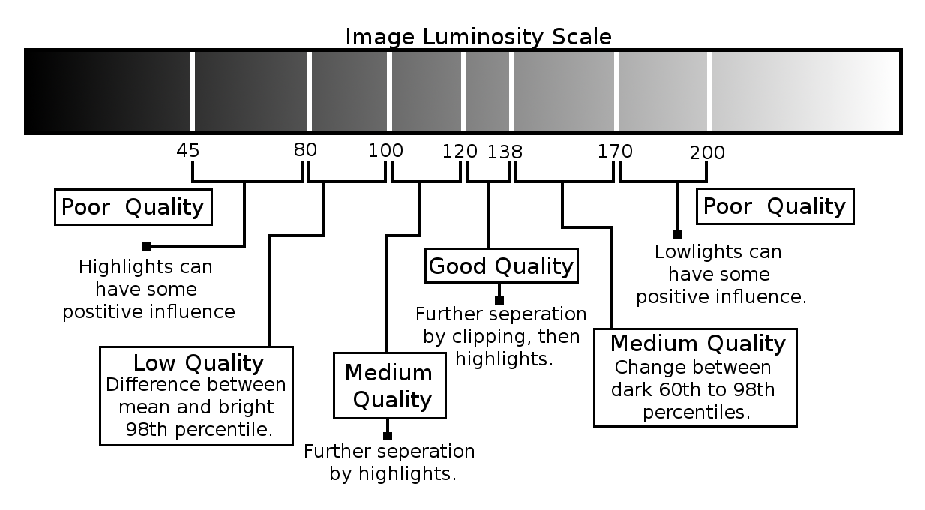
\includegraphics[scale=0.53,clip]{imageluminosity.eps}\
    \label{exposurefigure}
  \caption{The Exposure process: This figure shows the inital segmentation of images by mean (values 0 to 255), then the further segmentation of images of medium and good quality (mean ranges 100-120, and 120-138 respectively).}
\end{figure}
Image exposure is a measure of how approproate the lighting is in a given image.  While traditionally measured in-camera with light meter over the area, our exposure algorithm evaluates how the lighting in the result image appears to a human observer.  Images are ranked according to various measures of their luminosity.  Luminosity is a measure of how bright the human visual system perceives a color. As the human eye is most sensitive to green and red ranges, those color portions are weighted more heavily to a color's overall perceived intensity. The calculation used by the exposure analyst is
\[
p=.59r+.3g+.11b
\]
where \(p\) is the perceived intensity, and \(r\), \(g\), and \(b\) are the red, green, and blue components, respectively(XX THIS FORMULA NEEDS REFERENCE).

Based on the idea that the the mean value of image luminosity is an approximate indication of how well-exposed an image is, images are first segmented based on their average luminosity value.

The categories of mean luminosity value (“mean”) correspond roughly to a parabolic mapping of exposure values, with well exposed photographs having a mean of \(130<p<140\): the further towards the extreme high and low means, the worse quality the image is. These divisions are used as the starting point of analysis. Within each category, different measures indicate either a positive or negative overall impact on image quality, which impact depends upon the various categories. For example, in an overall dark mean, having more extreme bright areas makes the image more balanced, while in a bright image they usually indicate that it has been overexposed.

The other measures of image quality are also based on luminosity, and were determined by taking various measurements on a deliberately chosen pool of images that had a wide variety of exposure problems. The measures are as follows: clipping, highlights, lowlights, the upper 60th and 98th percentiles, the lower 60th and 98th percentiles, and variance. Each of these measures are calculated on both the foreground and the background of the image, relative to the area over which they are calculated.

Overexposure of an image can lead to large areas in the photo in which the human eye cannot discern any form (note that this definition can also indicate areas of a solid white value that contains absolutely no data about the form present). However, as the program is primarily concerned about how humans perceive images, the number of pixels in the highest five perceived values are used to calculate the “highlights” present in the image.

Lowlights can be caused by underexposure, but they can also be a product of poor lighting (e.g., photographing a shadowed object in extremely bright conditions). Again, some lowlights are desirable for contrast in an image, but too much leads to an undecipherable image.

Clipping is an indication of how much information loss there is in the image due to extreme shadows and bright spots, measured as a sum of the Highlights and Lowlights.

The percentiles of the image are determined for both the bright and the dark sides of luminosity. For example, to calculate the lower 60th percentile, the value is found at which the sum of the number of pixels that are darker than the given value is equal to sixty percent of the pixels in the image. The upper percentiles are found by the summation of the pixels that are brighter than the given value. These four measures give a good indication of the spread of the luminosity, e.g., how sharp the transitions between the extreme and middle values are.

The most extreme mean luminosity values are images of very poor quality, and are rated as such based solely on the mean value, although having a bright 98th high percentile can provide enough contrast to make a discernible image, though certainly nothing of quality. Means between 80 and 170 encompass nearly all images of medium through excellent exposure, and thus require the most analysis. After being subdivided into mean categories, they are again subdivided into further categories (see figure \ref{exposurefigure}) before analysis.

\subsection{Color Harmony}   
\begin{figure}[t]
  \centering
    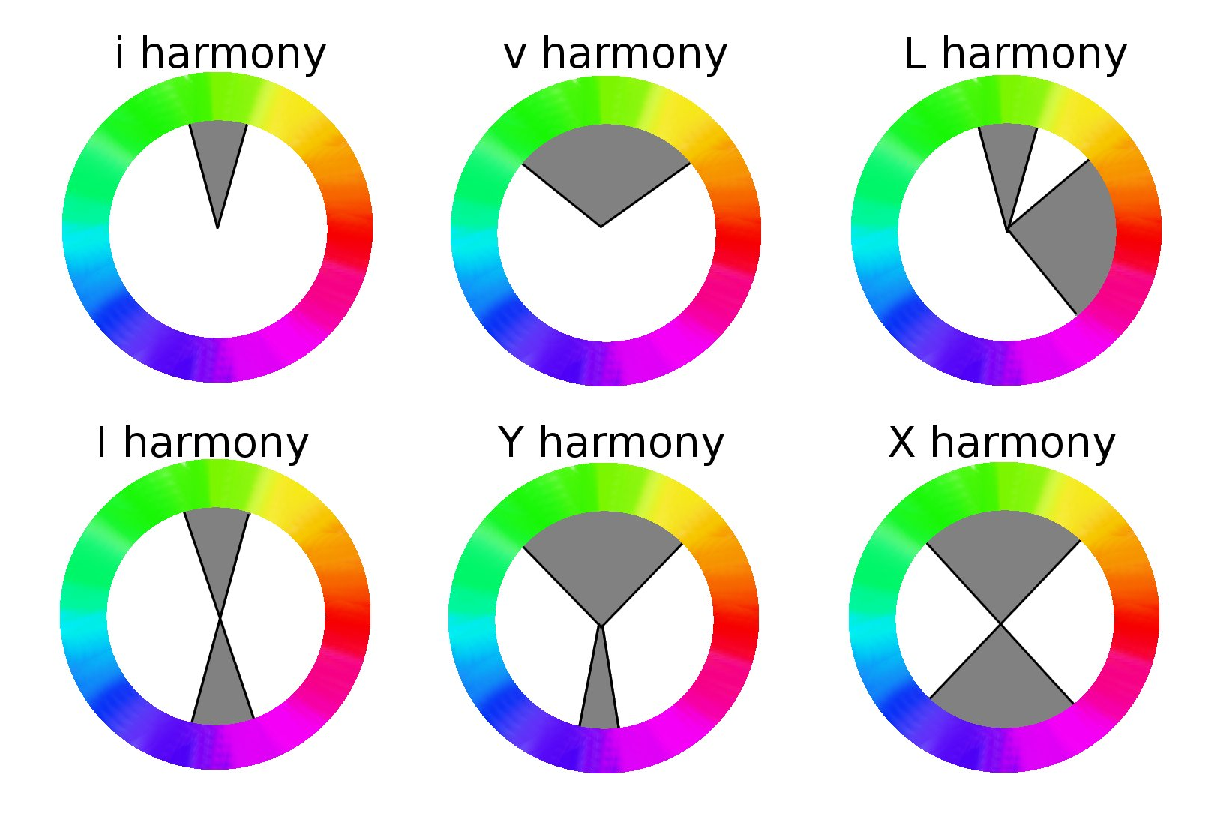
\includegraphics[scale=0.38,clip]{colorharmony.eps}
  \caption{The harmonies described in \cite{COL:COL10004} are used to find the quality of the relationships between colors.}
\end{figure}

Based on the seven types of color harmonies described in \cite{Cohen-Or:2006:CH:1179352.1141933}, the "ColorCritic" module measures which types of harmony are present in a photograph. It uses the I,v,L,I,Y, and X type harmonies (T and N are omitted).

For each harmony type, the hue is found with the most occurrences of supporting harmony (other pixels that fall in the harmonic range) as well as the percent of the image that has harmonious pixels. Similar to the Exposure Analyst, ColorCritic divides it's images into several categories before further analysis. However, because people tend to like colorful, intense images (XX THIS NEEDS TO BE SUPPORTED WITH A REFERENCE- IF THE SAME AS COHEN, WE CAN JUST CITE THAT), ColorCritic divides the images by the color saturation in the image using the results from Mechanical Turk rankings to determine where the exact divisions are. The harmony types are used to differentiate between various qualities of images withing the saturation ranges.

The first harmony checked is the average and great image's I type. If there is a large amount of I harmony, the difference between I and Y harmonies is checked. Because I and Y overlap, you need to check how much of an increase if between the two. If it is very significant, Y harmony is most likely. When the difference is slight, you have a good I harmony (and thus high rating). If there is a medium difference, the I harmony is weak. Rating of the images can be determined on medium to great harmony. A similar check is done in X versus Y harmony. A last pass is done to check the L type on the great images, and a pass checking the v and i harmonies is done on the average images.

The poor images follow a similar path, starting with analysis by the X harmony, and ending with a pass done with i harmony.

\section{Results}
We have run our algorithm on several publicly available datasets as well as our own. We used Amazon Mechanical Turk and gathered a total of 454 (XX  ADD QUALITY FILTER) users rankings across trials.

Enumerated below are the results and comparisons to similar works.

\subsection{Quality Filtering} When asking a user to choose which images to keep and which to discard, our algorithm correctly discarded XX\% of the images, and incorrectly discarded XX\%. When limiting both the algorithm and the user to discarding a fixed number of chronological photographs (ten out of twenty), we improved these numbers to XX\% accuracy with XX\% false-negatives. (XX WE PROBABLY ONLY HAVE TIME TO GATHER THE SECOND NUMBER- FIXED NUMBER OF DISCARDS)

\subsection{Image Rating} Separate trials were run to compare our algorithm to previously ranked images: 48 from \cite{1640788}, 100 from \cite{springerlink:10.1007/978-3-540-88690-7_29}, and 459 from our own data (XX DIDN'T WE DECREASE THE SIZE OF THIS? WE DON'T HAVE JULIE'S, ONLY ULA'S). Here we obtain an absolute, no-reference rating of each image.

We took a random sample of 100 images from the 11,981 images provided by \cite{springerlink:10.1007/978-3-540-88690-7_29}. We asked 44 Turk users to rank 50 images on a scale from one to ten.

\begin{figure}
  \centering
    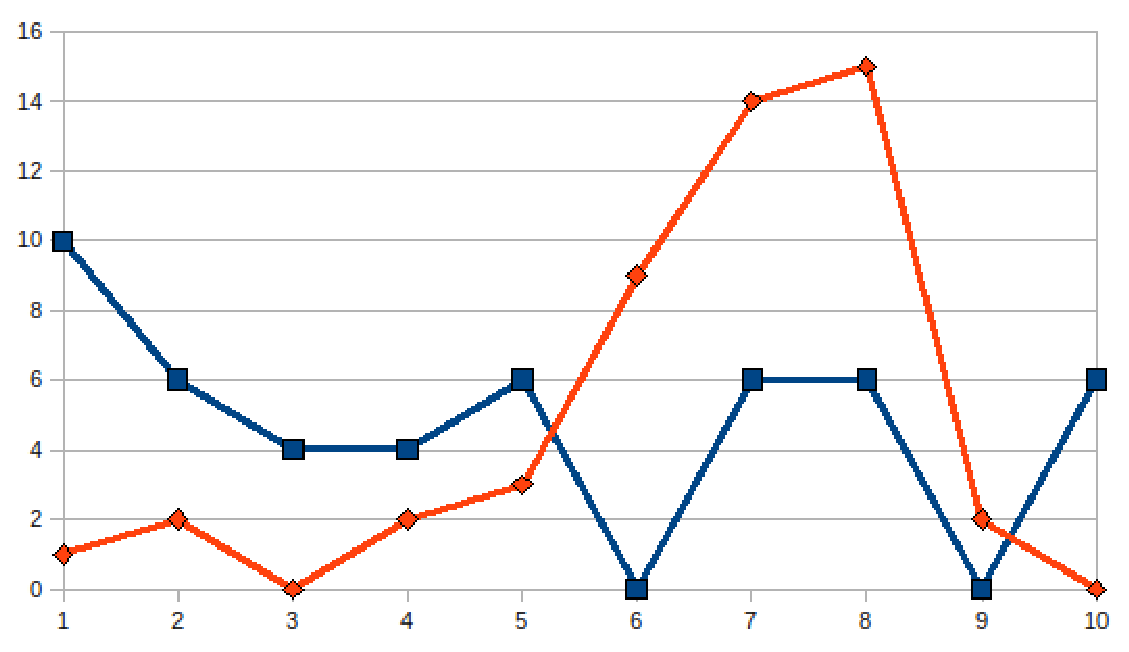
\includegraphics[scale=0.40,clip]{ke_vs_us.eps}
  \caption{X-axis: ten-point scaled rating.  Y-axis: number of images with this rating. We see that Ke's ratings do not match our ground truth. XX INACCURACY ASIDE, WE SHOULD MAKE THIS WORK FOR B\&W AND MAYBE LABEL AXES ON ACTUAL CHART?}
  \label{fig:ke_vs_us}
\end{figure}
When comparing Ke's data set, we see that their ground truth is based on different factors (Fig.~\ref{fig:ke_vs_us}). Whereas our work matches Amazon Mechanical Turk users' ratings with an accuracy of 80\%, Ke's only matches it with an accuracy of 45\%. Here, accuracy is defined as being within one standard deviation of the users' rankings.

XX INSERT DATA FOR OTHER DATA SET

\subsection{Binary Classification} Using the same data as the Image Rating trials, we have found that our algorithm can distinguish between professional and non-professional images well. Barsky \cite{Yeh:2010:PPR:1873951.1873963} and Luo \emph{et. al}\cite{springerlink:10.1007/978-3-540-88690-7_29} obtained 96\% accuracy when classifying images into the two categories. When classifying "non-professional" as ratings below XX and "professional" as ratings above XX, our rating system matches a user's with XX\% accuracy.

\section{Conclusion and Future Work}
We propose a method of applying current research to automate another step of the Photographer's Process. By focusing on obtaining an ordering which is representative of all photographs taken, we obtain a diverse set of high quality images similar to what a user would have chosen manually. We derive a novel algorithm for analyzing exposure quality. We improve upon previous algorithms which find temporal gaps between images to obtain a metric for temporal nearness. The final ordering depends on both the quality ranking and the number of similar images which have already appeared.

Our work focuses on a small portion of the Photographer's Process. In the future, we would like to see the idea of relative rankings applied to the second Retouching step. (It has already been extensively applied to the third Retrieval step.) Retouching can use relative processing to increase creativity between similar images or combine data from multiple images. With this, we would be able to automate the Photographic Process.
\bibliographystyle{plain}
\bibliography{README_BIB}
\end{document}
